% Chapter 13 -- Value at Risk and Its Backtests
% Requires: amsmath, amssymb, booktabs, array, tabularx, graphicx, tcolorbox (breakable, skins), hyperref or url.
% Defines the callout box only if the preamble has not.
\providecolor{fenavy}{HTML}{1B2A6B}
\providecolor{feshade}{HTML}{F3F5FA}
\makeatletter
\@ifundefined{callout}{%
  \newtcolorbox{callout}{breakable, enhanced,
    colback=white, colframe=gray!70, boxrule=0.5pt, arc=1mm,
    borderline west={2.5pt}{0pt}{gray!70},
    left=8pt, right=8pt, top=4pt, bottom=4pt}%
}{}
\makeatother

\chapter{Value at Risk and Its Backtests}
\label{ch:13}

Value at Risk compresses the risk of a portfolio into one number: the loss that should be exceeded only on a stated fraction of days. A bank that reports a one-day 99\% VaR of \$50 million is claiming that it will lose more than \$50 million on about one trading day in a hundred. From the mid-1990s that number set banks' capital requirements for market risk, and it still appears in every large bank's annual report.

VaR is unusual among the claims in this book because it is a \emph{forecast that checks itself}. Every day produces a test: either the loss exceeded the VaR or it did not. Over a few years the breaches accumulate into a record that anyone can test. The regulators built exactly such a test into the rules.

The record is mixed. Chapter 11 showed that volatility can be forecast. This chapter asks whether those forecasts, turned into VaR, deliver what they promise: the right number of breaches, at the right times, in crises as well as in calm markets.

By the end of the chapter you will be able to:

\begin{itemize}
  \item compute a parametric VaR and expected shortfall, and scale them across horizons with the square-root-of-time rule, knowing when it fails;
  \item explain coherence and show with an example how VaR can fail subadditivity;
  \item compare parametric, historical simulation, GARCH and filtered historical simulation VaR models;
  \item state the claim of conditional coverage and summarize the evidence from banks and from model comparisons;
  \item backtest a VaR model with the Kupiec and Christoffersen tests and the Basel traffic light, and backtest expected shortfall;
  \item judge a bank's or fund's risk disclosures and know what VaR cannot tell you.
\end{itemize}

\section{Foundations: VaR, expected shortfall and their properties}
\label{sec:13-foundations}

\textbf{Value at Risk.} For a confidence level $1 - \alpha$ and a horizon (one day, ten days), VaR is the loss that is exceeded with probability $\alpha$:
\begin{equation}
  P(\text{Loss} > \mathrm{VaR}) = \alpha
  \label{eq:13-var}
\end{equation}
It is a \textbf{quantile} of the loss distribution. A 99\% one-day VaR is the 1st percentile of tomorrow's return, with the sign flipped. If daily returns are normal with mean zero and standard deviation $\sigma$, then $\mathrm{VaR} = z\sigma$, where $z = 1.645$ at 95\%, 2.326 at 99\% and 3.090 at 99.9\%.

\textbf{Expected shortfall (ES)}, also called conditional VaR, is the average loss on the days when the VaR is exceeded:
\begin{equation}
  \mathrm{ES} = E[\text{Loss} \mid \text{Loss} > \mathrm{VaR}]
  \label{eq:13-es}
\end{equation}
For a normal distribution, $\mathrm{ES} = \sigma\,\phi(z)/\alpha$, where $\phi$ is the normal density. ES always exceeds VaR at the same confidence level. VaR says where the tail starts. ES says how bad the tail is (Figure~\ref{fig:13-var-es}).

\begin{figure}[htbp]
\centering
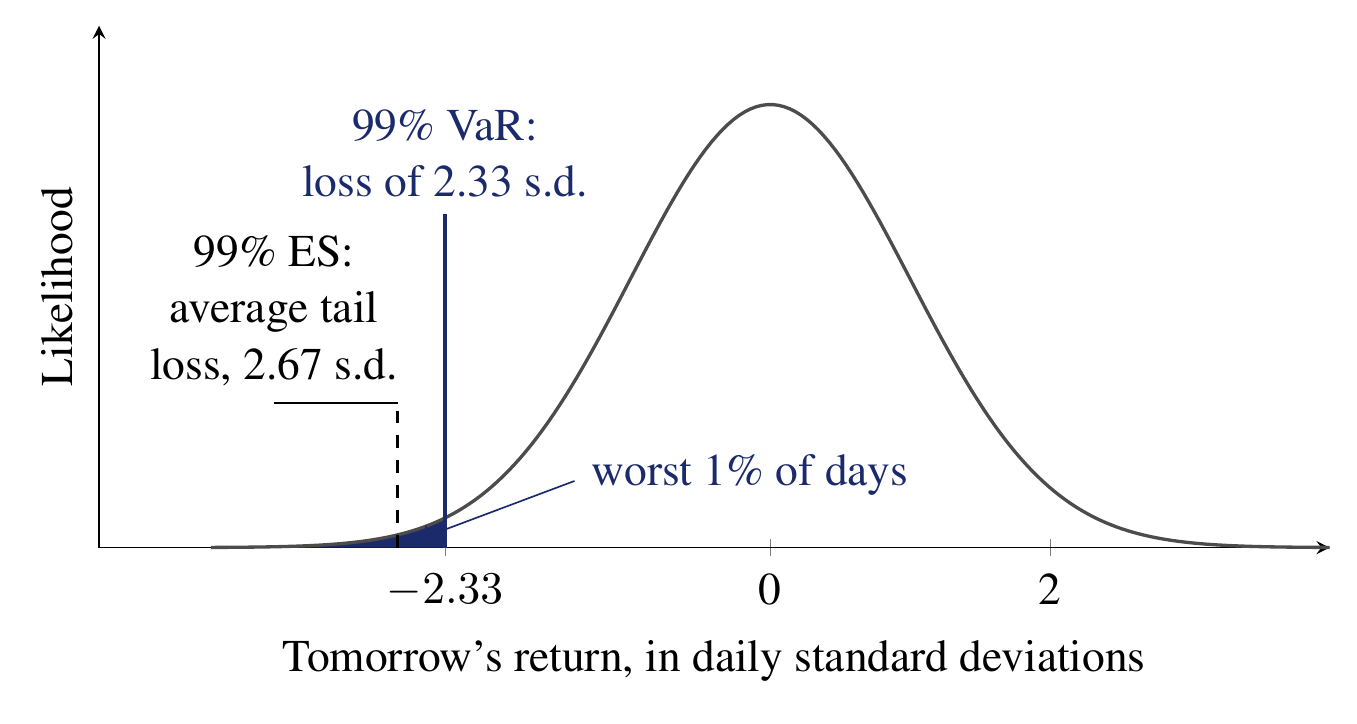
\includegraphics[width=0.85\linewidth]{images/fig13-1-var-es.png}
\caption{VaR and expected shortfall for normal returns. The 99\% VaR marks where the worst 1\% of days begins, 2.33 standard deviations below zero. The 99\% ES is the average loss within that tail, 2.67 standard deviations.}
\label{fig:13-var-es}
\end{figure}

\textbf{Coherence.} Artzner, Delbaen, Eber and Heath (1999) listed four properties a sensible risk measure should have. The one VaR can violate is \textbf{subadditivity}: the risk of a combined portfolio should not exceed the sum of the risks of its parts, since diversification should not add risk. ES is subadditive; VaR is not in general. VaR is subadditive for normal returns, so the failure shows up in portfolios with very skewed payoffs, such as credit and options.

\textbf{Square-root-of-time.} If daily returns are independent with the same variance, the $h$-day standard deviation is $\sqrt{h}$ times the daily one, so a 10-day VaR is about $\sqrt{10} \approx 3.16$ times the one-day VaR. Volatility clustering (Chapter 11) breaks the assumption: after a calm period the rule overstates risk, and after a shock it understates it.

\textbf{Methods.} The three main families of VaR models are set out in Section~\ref{sec:13-how}:

\begin{itemize}
  \item \emph{parametric}, which assumes a distribution and estimates $\sigma$;
  \item \emph{historical simulation}, which uses the empirical quantile of past returns;
  \item \emph{Monte Carlo}, which simulates from a model of the risk factors.
\end{itemize}

\textbf{Worked example.} A \$10 million position in a stock index has a daily volatility of 1.2\%.

\begin{itemize}
  \item Normal 99\% one-day VaR $= 2.326 \times 1.2\% \times \$10\text{m} \approx \$279{,}000$.
  \item Normal 99\% ES $= 1.2\% \times \phi(2.326)/0.01 \times \$10\text{m} = 2.665 \times 1.2\% \times \$10\text{m} \approx \$320{,}000$.
  \item Normal 97.5\% ES $= 2.338 \times 1.2\% \times \$10\text{m} \approx \$281{,}000$, almost the same as the 99\% VaR. This is why regulators chose 97.5\% when they moved from VaR to ES.
  \item 10-day VaR by the square-root rule: $\sqrt{10} \times \$279{,}000 \approx \$883{,}000$.
  \item With 500 days of history, the 99\% historical-simulation VaR is the loss between the 5th and 6th worst days.
\end{itemize}

\textbf{Subadditivity failure.} Two bonds each default with probability 4\%, losing 100 if they do and nothing otherwise. Each bond's 95\% VaR is 0, since default is less likely than 5\%. For a portfolio of both, with independent defaults, the probability of at least one default is $1 - 0.96^2 = 7.84\%$, so the portfolio's 95\% VaR is 100. Diversifying has \emph{increased} the measured risk.

\textbf{Further reading.} Hull, \emph{Risk Management and Financial Institutions} and \emph{Options, Futures, and Other Derivatives} (VaR and ES, historical simulation, model-building approach, backtesting); Jorion, \emph{Value at Risk: The New Benchmark for Managing Financial Risk}; McNeil, Frey and Embrechts, \emph{Quantitative Risk Management} (risk measures, coherence, backtesting); Christoffersen, \emph{Elements of Financial Risk Management} (VaR models and backtests).

\section{How it works}
\label{sec:13-how}

Every VaR model answers two questions: how volatile will tomorrow be, and what shape does the tail have? The models in this chapter combine different answers.

\begin{center}
\small
\begin{tabularx}{0.9\linewidth}{@{}>{\raggedright\arraybackslash}p{0.28\linewidth}>{\raggedright\arraybackslash}X>{\raggedright\arraybackslash}X@{}}
\toprule
Model & Volatility & Tail shape \\
\midrule
Normal, rolling window & Equal-weighted past window (here 250 days) & Normal \\
Historical simulation (HS) & Implicit in the window & Empirical quantile of past returns \\
EWMA (RiskMetrics) & Exponentially weighted, $\lambda = 0.94$ & Normal \\
GARCH & Estimated, mean-reverting & Normal \\
GJR-GARCH with Student-$t$ shocks & Estimated, with leverage effect & Student-$t$, estimated \\
Filtered historical simulation (FHS) & GJR-GARCH & Empirical quantile of past \emph{standardized} returns \\
\bottomrule
\end{tabularx}
\end{center}

\textbf{Historical simulation} is the most popular method at banks (P\'erignon and Smith 2010) because it needs no distributional assumption and handles nonlinear positions, such as options, by revaluing the portfolio under each past day's market moves. Its weakness is slowness. A 250-day window gives the same weight to a crash eleven months ago as to yesterday's, and none at all to one twelve months and a day ago. When volatility jumps, HS VaR responds only as the new large losses enter the window. When they leave, it drops abruptly.

\textbf{EWMA and GARCH} respond to volatility within days, which is Chapter 11's central finding. But with normal shocks they understate the tail. Even after volatility clustering is removed, standardized daily returns have fatter tails than the normal distribution, so a normal 99\% VaR built on a good volatility forecast is still breached too often.

\textbf{Filtered historical simulation} (Barone-Adesi, Giannopoulos and Vosper 1999; Hull and White 1998) combines the two strengths. It divides each past return by the volatility forecast for that day, giving standardized returns that are roughly independent and identically distributed. It takes their empirical quantile, which captures the fat tails without assuming a distribution, and multiplies by today's volatility forecast. The GJR-$t$ model does the same with a parametric tail.

A VaR model can fail in two distinct ways. It can be \textbf{wrong on average}, breached on 2\% of days instead of 1\%. Or it can be \textbf{right on average but wrong at the wrong times}, with breaches bunched in a few turbulent weeks. The second failure is the more dangerous, because the bunched breaches arrive exactly when capital is scarce. The backtests in Section~\ref{sec:13-backtest} test for both.

\section{The claim}
\label{sec:13-claim}

\begin{callout}
\textbf{Claim.} A well-built 99\% one-day VaR model is breached on about 1\% of trading days, and its breaches are independent over time. Breaches neither cluster in turbulent periods nor become more likely after a breach.
\end{callout}

This is the claim implicit in every VaR number a bank reports and in the Basel rules that used VaR to set capital. Christoffersen (1998) called the two parts \textbf{unconditional coverage} and \textbf{independence}. Together they form \textbf{conditional coverage}: on each day, given everything known the day before, the probability of a breach is exactly 1\%.

To test it we need to be precise on four points.

\begin{itemize}
  \item \textbf{Which models.} The claim is not that any VaR model works. It is that some models, built on the evidence of Chapter 11, can achieve conditional coverage. We test six, from the simplest to filtered historical simulation.
  \item \textbf{Which portfolio.} The lab uses the U.S. stock market, a single liquid position with daily data back to 1926. Bank portfolios are more complex, and their own backtests (Section~\ref{sec:13-evidence}) are the stronger test of practice.
  \item \textbf{Which confidence level.} The claim is stated at 99\%, the Basel level, but a model that is right at 99\% and badly wrong at 99.9\% is of limited use for the tail events that matter.
  \item \textbf{What would count against it.} The claim fails for a model if its breach rate differs significantly from 1\%, or if breaches are significantly clustered. It weakens if every model fails in crises, even those that pass over the full sample.
\end{itemize}

\section{The original evidence}
\label{sec:13-evidence}

\textbf{RiskMetrics and the Basel rules.} In 1994 J.P. Morgan published its RiskMetrics methodology and data free of charge. Its daily volatilities used the EWMA rule with $\lambda = 0.94$, and its VaR assumed normal returns. The fourth edition of the \emph{Technical Document} (1996) became the reference for the industry. In 1996 the Basel Committee allowed banks to use their own VaR models to set capital for market risk: a 99\% ten-day VaR, multiplied by at least 3. The multiplier rises with the number of breaches in a 250-day backtest, the \textbf{traffic light} described in Section~\ref{sec:13-backtest}. VaR thus became both a management tool and a regulatory one, and the backtest became a test with consequences.

\textbf{The statistics of backtesting.} Kupiec (1995) proposed testing whether the breach rate equals the stated probability, and showed how little power the test has over a single year: at 99\% only 2.5 breaches are expected in 250 days, so even a badly wrong model is hard to reject. Christoffersen (1998) added the test of independence and combined the two into the conditional-coverage test.

\textbf{Banks' own VaR.} Berkowitz and O'Brien (2002) obtained daily VaR forecasts and trading results for six large U.S. banks. The banks' 99\% VaRs were generally \emph{conservative}, breached less than 1\% of the time. But the breaches that did occur clustered, most of them in the turmoil of August to October 1998. A simple GARCH model of each bank's total trading P\&L performed about as well as the banks' detailed models and responded faster to changes in volatility. P\'erignon and Smith (2010) found that historical simulation was by far the most popular method among banks, and that historical-simulation VaR contained very little information about future volatility.

\textbf{Model comparisons.} Studies that backtest many models on index returns reach a consistent conclusion. Methods that combine a GARCH-type volatility forecast with a fat-tailed or empirical distribution of standardized returns perform best. Plain historical simulation and normal models with slow-moving volatility perform worst (Kuester, Mittnik and Paolella 2006). McNeil and Frey (2000) proposed the conditional extreme-value approach and the exceedance-residual test of expected shortfall used in this chapter's lab.

\section{Backtesting VaR and expected shortfall}
\label{sec:13-backtest}

A backtest compares each day's VaR forecast, made the day before, with that day's actual loss. A \textbf{breach} (or exception) is a day on which the loss exceeded the VaR. The breach sequence, a string of 0s and 1s, is the raw material for every test.

\textbf{Unconditional coverage (Kupiec 1995).} With $n$ days and $x$ breaches, the likelihood-ratio statistic compares the observed rate $x/n$ with the stated probability $\alpha$:
\begin{equation}
  LR_{uc} = -2\ln\!\left[(1 - \alpha)^{n-x}\,\alpha^{x}\right] + 2\ln\!\left[\left(1 - \tfrac{x}{n}\right)^{n-x}\left(\tfrac{x}{n}\right)^{x}\right]
  \label{eq:13-kupiec}
\end{equation}
Under the null hypothesis it has a $\chi^2$ distribution with one degree of freedom. It rejects both too many breaches (risk understated) and too few (capital wasted).

\textbf{Independence (Christoffersen 1998).} Estimate two probabilities: of a breach after a day without one ($\pi_{01}$), and of a breach after a breach ($\pi_{11}$). If breaches are independent, they are equal. The likelihood-ratio test of $\pi_{01} = \pi_{11}$ is $\chi^2(1)$. Adding $LR_{uc}$ gives the conditional-coverage test, $\chi^2(2)$. For a correct 99\% model, $\pi_{11}$ should be about 1\%. Values of 5\% to 10\% mean the model reacts too slowly to turbulence.

\textbf{The Basel traffic light.} Regulators count breaches of the 99\% one-day VaR over the most recent 250 trading days (Figure~\ref{fig:13-traffic}):

\begin{center}
\small
\begin{tabularx}{0.9\linewidth}{@{}>{\raggedright\arraybackslash}p{0.12\linewidth}>{\raggedright\arraybackslash}p{0.16\linewidth}>{\raggedright\arraybackslash}p{0.22\linewidth}>{\raggedright\arraybackslash}X@{}}
\toprule
Zone & Breaches & Capital multiplier & Probability of this many or fewer for a correct model \\
\midrule
Green & 0--4 & 3.0 & 89.2\% \\
Yellow & 5--9 & 3.40 to 3.85 & 99.99\% at 9 \\
Red & 10 or more & 4.0 & n/a \\
\bottomrule
\end{tabularx}
\end{center}

\begin{figure}[htbp]
\centering
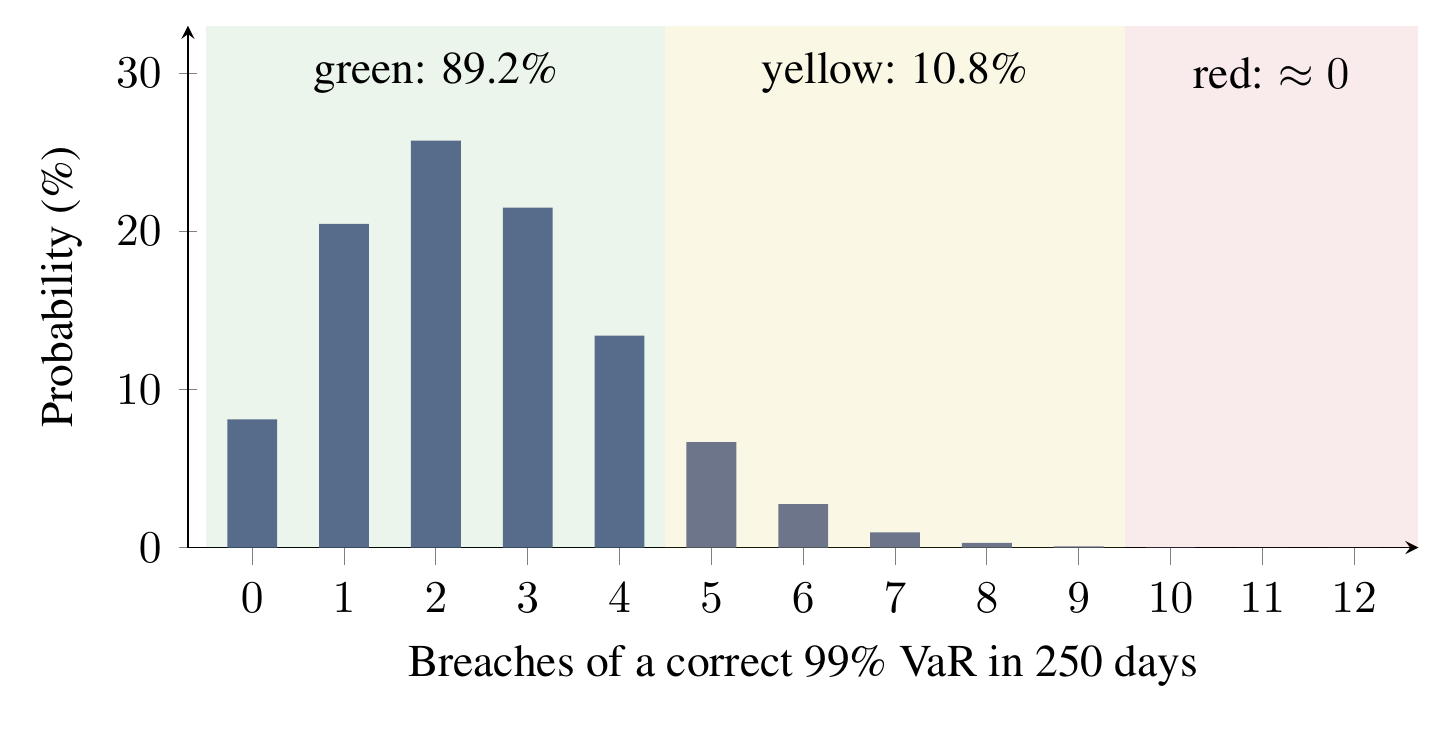
\includegraphics[width=0.85\linewidth]{images/fig13-2-traffic-light.png}
\caption{The Basel traffic light. The bars give the probability that a correct 99\% VaR model is breached a given number of times in 250 days. It lands in the green zone 89.2\% of the time and in the yellow zone 10.8\% of the time, and almost never in the red.}
\label{fig:13-traffic}
\end{figure}

A correct model lands in the yellow zone about one year in nine and almost never in the red. The zones were designed to balance two errors: penalizing banks with good models and letting banks with bad models through.

\textbf{Expected shortfall.} In 2016 the Basel Committee's Fundamental Review of the Trading Book replaced 99\% VaR with 97.5\% ES for setting market-risk capital, because ES captures the size of tail losses and is subadditive. ES is harder to backtest. Gneiting (2011) showed that ES, unlike VaR, is not \textbf{elicitable}: no scoring function is minimized by the true ES, so forecasts cannot be ranked by average loss as VaR forecasts can. Backtests exist nonetheless. The \textbf{exceedance-residual test} of McNeil and Frey (2000) checks whether, on breach days, the loss beyond the ES averages zero. Acerbi and Sz\'ekely (2014) proposed further tests. The Basel framework still backtests VaR at 97.5\% and 99\% alongside the ES used for capital.

\section{Replication lab: ninety-five years of VaR backtests}
\label{sec:13-lab}

\begin{callout}
\textbf{Lab 13 at a glance.} \emph{Claim on trial:} a well-built 99\% VaR model achieves conditional coverage. \emph{Data:} daily U.S. market returns (Mkt-RF + RF from the Kenneth French library) from 1930 to the present, about 24,000 trading days; free. \emph{Code:} runs as a script (\texttt{python lab13.py}) or as a notebook with a prediction prompt before each step.
\end{callout}

Lab 13 backtests the six models of Section~\ref{sec:13-how}. Every forecast uses only data up to the day before. The GARCH models are re-estimated once a year on the previous ten years.

\textbf{Part A, coverage.} For each model at 99\%: breaches against the roughly 240 expected, Kupiec and Christoffersen tests, average VaR, the worst loss as a multiple of the VaR, and the share of calendar years that would have fallen in the Basel yellow and red zones. Figure 13.3 shows two models through 2007--2010, and Figure 13.4 compares breach rates.

\textbf{Part B, clustering.} The probability of a breach after a breach, and breaches per year against the Basel zones (Figure 13.5).

\textbf{Part C, stress tests.} Breaches in four crises; the ratio of actual to expected breaches at confidence levels from 95\% to 99.9\% (Figure 13.6); and historical simulation with one, two and four years of data.

\textbf{Part D, expected shortfall.} At 97.5\%, the ratio of the average loss on breach days to the average ES forecast, and a test of whether exceedance residuals, scaled by volatility, average zero (Figure 13.7).

The lab tests the claim in its simplest setting: a single linear position in a liquid market with a long history. A bank's trading book adds options, credit and illiquid positions, and those make every model harder to build. If the models struggle here, they will not do better there.

\textbf{What the simulated run shows.} The simulation draws returns from a GJR-GARCH model with Student-$t$ shocks, so the GJR-$t$ model is the true model. It passes every test: 1.01\% breaches at 99\%, a breach probability after a breach of 0.8\%, and an ES ratio of 1.00. Filtered historical simulation is nearly as good. The normal and historical-simulation models are breached about twice as often as they should be, with strong clustering, and they understate ES. These results confirm that the code and the tests work. They say nothing about real markets. Run the lab on the real data to reach your own verdict.

\section{Stress tests}
\label{sec:13-stress}

\textbf{Crises.} The full-sample breach rate can hide disastrous weeks. On October 19, 1987, the Dow Jones Industrial Average fell 22.6\%, its largest one-day percentage loss. No model calibrated on the calm months before could have put that inside a 99\% VaR. Part C counts breaches in 1930--32, October 1987, the autumn of 2008 and the spring of 2020. A correct 99\% model should average about 0.2 breaches in a 22-day month. Expect every model to exceed that in these windows. The question is how many breaches each produces and how quickly it adapts.

\textbf{Confidence level.} Fat tails punish models more the further into the tail they go. Under the normal distribution a 99.9\% loss is only 1.33 times a 99\% loss ($3.09/2.33$). In equity returns the ratio is larger. Normal-based models that are slightly off at 95\% can be several times off at 99.9\% (Figure 13.6). The test also has very little power at 99.9\%: about 24 breaches are expected in 95 years, so a single bad week moves the ratio noticeably.

\textbf{Window length.} A short historical-simulation window adapts faster but estimates the 1\% quantile from very few observations: with 250 days, only two or three. A long window is more stable but slower to react after a calm period. Part C compares 250, 500 and 1,000 days. The choice moves the breach rate but does not fix clustering, since no equal-weighted window responds to volatility the way GARCH does.

\textbf{Procyclicality.} A VaR that responds quickly to volatility, as GARCH and EWMA do, raises capital requirements and forces deleveraging in exactly the weeks when markets are falling. That is good risk measurement but can amplify a crisis if every bank does it at once. A slow VaR, such as long-window historical simulation, is less procyclical but is breached in clusters. Basel 2.5 (2009) added a \textbf{stressed VaR}, calibrated to a year of significant stress, partly to make capital less dependent on recent calm.

\section{Verdict}
\label{sec:13-verdict}

\begin{callout}
\textbf{Verdict: weakens} (as of October 2026). The claim holds for the right models in normal times: VaR models that combine a responsive volatility forecast with a fat-tailed distribution come close to 1\% breaches at 99\% with little clustering over long samples. It fails for the models most widely used in practice, normal and plain historical simulation, which are breached in clusters. It fails for every model in the first days of a crisis and deep in the tail.
\end{callout}

What survives:

\begin{itemize}
  \item \textbf{Coverage is achievable.} Filtered historical simulation and GARCH models with fat-tailed shocks deliver close to the stated breach rate over long samples, in the literature and in tests like the lab's. The tools of Chapter 11 work.
  \item \textbf{Backtesting works as designed.} The Kupiec and Christoffersen tests, and the Basel traffic light, separate good models from bad ones over long samples. A model that clusters its breaches is caught.
\end{itemize}

What weakens it:

\begin{itemize}
  \item \textbf{Practice lags the evidence.} Historical simulation, the most popular method at banks, reacts slowly and contains little information about future volatility (P\'erignon and Smith 2010). Its breaches cluster in exactly the periods when losses matter.
  \item \textbf{Crises break every model.} No model built on past data anticipates the first day of a crash. In October 1987, in 2008 and in March 2020 breaches came in bunches.
  \item \textbf{The tail beyond 99\% is poorly measured.} Breach rates at 99.9\% are worse for most models, and the tests have little power to tell.
  \item \textbf{VaR says nothing about the size of the loss beyond it.} A model can pass every VaR backtest while understating how bad the bad days are. Expected shortfall addresses this, but it inherits the same volatility forecasts and is harder to backtest.
\end{itemize}

The verdict would move to \emph{survives} if the models used in practice achieved conditional coverage through crises, which would require volatility forecasts faster than any yet built from daily data. It would move to \emph{fails} if even the best models failed coverage tests over long samples, which the evidence so far does not show.

\section{What practitioners and investors can use}
\label{sec:13-investors}

\textbf{For anyone measuring risk:}

\begin{itemize}
  \item \textbf{Use a responsive volatility forecast.} EWMA at the least, GARCH-type models for better results. A one-year equal-weighted window is too slow.
  \item \textbf{Use fat tails.} Scale standardized returns by an empirical or Student-$t$ distribution rather than the normal. Filtered historical simulation does both and is easy to implement.
  \item \textbf{Report ES alongside VaR,} and look at the largest losses directly, not only at percentiles.
  \item \textbf{Backtest continuously.} Count breaches, and also check whether they cluster. A model with the right number of breaches all in one month is not a good model.
  \item \textbf{Stress test separately.} VaR describes ordinary bad days. Scenarios such as a repeat of October 1987, 2008 or 2022 describe the days that threaten survival, and no backtest on recent data covers them.
\end{itemize}

\textbf{For investors reading a bank's or fund's risk disclosures:}

\begin{itemize}
  \item What method produces the VaR, and over what window? A historical simulation with a one-year window will look reassuring after a calm year.
  \item How many backtesting exceptions were there last year, and when did they occur?
  \item What is the stressed VaR or the worst scenario loss, relative to the reported VaR?
  \item What positions are hard to value daily? Their risk may not appear in the VaR at all.
\end{itemize}

\begin{callout}
\textbf{What Failed: bank VaR in 2007--08.} By 2007 large banks' trading risk was measured mainly by VaR and stress tests, and their market-risk capital was based on VaR. The Swiss Federal Banking Commission's investigation of UBS, the bank with the largest subprime losses in Europe, found that its super-senior CDO tranches had been judged ``VaR neutral,'' so they ``were not reflected in key internal risk reports.'' The AAA ratings fed straight into the risk metrics. Risk models, including VaR, ``operated on the basis of overoptimistic assumptions,'' and stress scenarios were ``too optimistic'': ``The real shocks proved to be far greater than any shocks anticipated.'' UBS's own report to shareholders recorded that the super-senior positions, which the desk had treated as fully hedged with protection on only a small part of their value, accounted for about half of the bank's losses by the end of 2007.

The failure was not that VaR was computed wrongly. It was that VaR measured the risk of positions that looked safe in recent data and could not see the risk of a market that had never been stressed. The regulatory response was the stressed VaR of Basel 2.5 and, later, the move to expected shortfall. In March 2020, regulators faced the opposite problem: banks' backtesting exceptions jumped with market volatility, and the Federal Reserve and other U.S. agencies excluded exceptions from March 6 to March 27, 2020, from the count, judging that they reflected ``widespread and unusual volatility'' (Board of Governors of the Federal Reserve System 2021).
\end{callout}

\section{Open questions}
\label{sec:13-open}

\begin{itemize}
  \item \textbf{Can intraday data fix the first day of a crisis?} Realized volatility from intraday returns (Chapter 11) responds faster than daily GARCH. Does it reduce breach clustering at the onset of crises?
  \item \textbf{How should ES be backtested and compared?} ES is not elicitable on its own, but it is jointly elicitable with VaR. Which tests have power at the sample sizes banks actually have?
  \item \textbf{Is risk measurement procyclical by design?} A VaR that responds quickly forces deleveraging in falling markets. How should risk measures balance accuracy against stability?
  \item \textbf{What about portfolios VaR handles badly?} Options, credit and illiquid assets have nonlinear or stale prices. How much worse are VaR backtests for them, and what replaces VaR there?
\end{itemize}

\section*{Exercises}
\addcontentsline{toc}{section}{Exercises}

\subsection*{Conceptual (all readers)}

\begin{enumerate}
  \item A \$5 million position has a daily volatility of 1.5\%. Compute the normal 95\% and 99\% one-day VaR, the 99\% ES and the 10-day 99\% VaR by the square-root rule.
  \item Using the two-bond example in Section~\ref{sec:13-foundations}, compute the portfolio's 95\% ES and show that ES is subadditive in this case.
  \item A bank reports 7 breaches of its 99\% VaR in 250 days. Compute the Kupiec statistic and p-value. Which Basel zone is it in, and what is the capital multiplier?
\end{enumerate}

\subsection*{Lab extensions (technical readers)}

\begin{enumerate}
  \setcounter{enumi}{3}
  \item Part A: which models pass the Kupiec test at 99\%? Which pass the Christoffersen independence test? Is there a model that passes one but not the other?
  \item Part B: for historical simulation, compute the average number of days between breaches and compare it with the 100 days expected. What does the distribution of durations tell you?
  \item Part C: count each model's breaches in October 1987. How many days did each model take before its VaR exceeded the losses of the following days?
  \item Part C: rerun the backtest at 99.9\%. Which models are within a factor of two of the expected breach rate? How confident can you be, given the number of breaches expected?
  \item Part D: do the models that pass the VaR backtest also pass the ES backtest? Is there a model that passes VaR but fails ES?
  \item A regulator proposes requiring all banks to use filtered historical simulation. Using the evidence in this chapter, write the case for and against, including the effect on procyclicality.
\end{enumerate}

\section*{References}
\addcontentsline{toc}{section}{References}

\begin{itemize}
  \item Acerbi, C. and Sz\'ekely, B. (2014). Back-Testing Expected Shortfall. \emph{Risk}, December 2014.
  \item Artzner, P., Delbaen, F., Eber, J.-M. and Heath, D. (1999). Coherent Measures of Risk. \emph{Mathematical Finance} 9(3): 203--228.
  \item Barone-Adesi, G., Giannopoulos, K. and Vosper, L. (1999). VaR without Correlations for Portfolios of Derivative Securities. \emph{Journal of Futures Markets} 19(5): 583--602.
  \item Basel Committee on Banking Supervision (1996). \emph{Supervisory Framework for the Use of ``Backtesting'' in Conjunction with the Internal Models Approach to Market Risk Capital Requirements}. Basel: Bank for International Settlements.
  \item Basel Committee on Banking Supervision (2009). \emph{Revisions to the Basel II Market Risk Framework}. Basel: Bank for International Settlements.
  \item Basel Committee on Banking Supervision (2016). \emph{Minimum Capital Requirements for Market Risk}. Basel: Bank for International Settlements.
  \item Berkowitz, J. and O'Brien, J. (2002). How Accurate Are Value-at-Risk Models at Commercial Banks? \emph{Journal of Finance} 57(3): 1093--1111.
  \item Board of Governors of the Federal Reserve System (2021). Banks' Backtesting Exceptions during the COVID-19 Crash: Causes and Consequences. \emph{FEDS Notes}, July 8.
  \item Christoffersen, P. F. (1998). Evaluating Interval Forecasts. \emph{International Economic Review} 39(4): 841--862.
  \item Gneiting, T. (2011). Making and Evaluating Point Forecasts. \emph{Journal of the American Statistical Association} 106(494): 746--762.
  \item Hull, J. and White, A. (1998). Incorporating Volatility Updating into the Historical Simulation Method for Value-at-Risk. \emph{Journal of Risk} 1(1): 5--19.
  \item J.P. Morgan/Reuters (1996). \emph{RiskMetrics---Technical Document} (4th ed.). New York: Morgan Guaranty Trust Company.
  \item Kuester, K., Mittnik, S. and Paolella, M. S. (2006). Value-at-Risk Prediction: A Comparison of Alternative Strategies. \emph{Journal of Financial Econometrics} 4(1): 53--89.
  \item Kupiec, P. H. (1995). Techniques for Verifying the Accuracy of Risk Measurement Models. \emph{Journal of Derivatives} 3(2): 73--84.
  \item McNeil, A. J. and Frey, R. (2000). Estimation of Tail-Related Risk Measures for Heteroscedastic Financial Time Series: An Extreme Value Approach. \emph{Journal of Empirical Finance} 7(3--4): 271--300.
  \item P\'erignon, C. and Smith, D. R. (2010). The Level and Quality of Value-at-Risk Disclosure by Commercial Banks. \emph{Journal of Banking \& Finance} 34(2): 362--377.
  \item Swiss Federal Banking Commission (2008). \emph{Subprime Crisis: SFBC Investigation into the Causes of the Write-downs of UBS AG}. Bern: SFBC.
  \item UBS AG (2008). \emph{Shareholder Report on UBS's Write-Downs}. Zurich: UBS.
\end{itemize}

\textbf{Data:} Kenneth R. French Data Library, Fama/French 3 Factors [Daily].
